\documentclass[]{../auvsi_doc}
\setkeys{../auvsi_doc.cls}{
	AUVSITitle={Capstone Team 45 Status Update 10/3/2018},
	AUVSILogoPath={./../logo.pdf}
}

\usepackage[toc,page]{appendix}

\begin{document}

\section{Goals for the Past Week}

The following is a list of our goals for the past week, as well as descriptions of their completion and/or progress:

\begin{enumerate}
\item \textbf{Finalize and ratify the Opportunity Development artifacts}\\
The project contract v1.0 has been completed, and is ready to submit to our Capstone instructor for initial review. The rest of the Opportunity Development artifacts are to be completed within the next couple of days.
\item \textbf{Investigate a Ubiquiti data link upgrade}\\
We have tested the new Ubiquiti rocket left for us from last year's team, and have determined that it provides adequate performance.
\item \textbf{Have the entire team focusing on implementing a mock competition with last year's system}\\
With the exception of a couple of team members fine-tuning the Opportunity Development artifacts, all team members are working towards getting last year's system up in the air.
\item \textbf{Investigate better options for a camera lens}\\
As it turns out, the camera had a lens filter attached to it, which didn't allow it to focus on far-off objects. Appendix~\ref{appendix:cameragraphic} illustrates a comparison of pixels per square inch (PPSI) for cameras of last year's teams. As the graphic shows, our camera setup falls on the low end of this spectrum. This is cause for looking into the matter more.
\item \textbf{Establish a wireless connection with the odroid computer}\\
We successfully completed this step, and even established a ROS network with the odroid communicating inertial data to a ground station on another machine.
\item \textbf{Modify the ground station to subscribe to raw images instead of compressed images}\\
After a little bit of research, we learned how to do this, but there are some minor hiccups which are currently being worked through. This will probably be completed by next week, but it's also not a super high priority at the moment.
\end{enumerate}

\section{Goals for the Coming Week}

The following is a list of our goals for the coming week, as well as details about how we plan to accomplish them:

\begin{enumerate}
\item \textbf{Finalize and ratify the Opportunity Development artifacts}\\
This will be done in correspondence with our Capstone instructor.
\item \textbf{Be ready to fly a mock competition (minus the camera) on Thursday of next week}\\
Based on the progress we've made, we are confident that, through consolidation of what each team member has learned through tinkering, we will be able to get a fully functional system by next week.
\item \textbf{Continue testing pixel resolution of our camera at large target distances}
\end{enumerate}

\textbf{Please send us any feedback with regards to the progress we've made, as well as our plans for the coming week.}

\newpage
\begin{appendices}

\section{Camera Resolution Comparisons}
\label{appendix:cameragraphic}
\begin{center}
	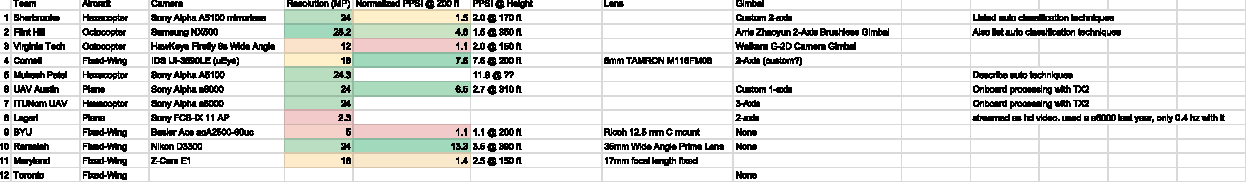
\includegraphics[width=\textwidth]{camera_graphic.pdf}
\end{center}

\end{appendices}

\end{document}
